\documentclass[a4paper,11pt,onecolumn,oneside,UTF8]{article}

\usepackage{ctex}     % 中文支持
\usepackage{amsthm,amsmath,amssymb}
\usepackage{mathrsfs}
\usepackage{bm}       % 公式中的粗体字符(用命令\boldsymbol)
\usepackage{graphicx, subfig}
\usepackage{caption}
\usepackage{float}
\usepackage{color}
\usepackage{enumerate}
\usepackage{multirow}
\usepackage{pgfplots}
\usepackage{tikz}
\usepackage{listings}
\usepackage[colorlinks,linkcolor=blue]{hyperref}

\addtolength{\topmargin}{-54pt}
\setlength{\oddsidemargin}{-0.9cm}  % 3.17cm - 1 inch
\setlength{\evensidemargin}{\oddsidemargin}
\setlength{\textwidth}{18.00cm}
\setlength{\textheight}{24.00cm}    % 24.62
\lstset{
 columns=fixed,       
 frame=none,                                          % 不显示背景边框
 backgroundcolor=\color[RGB]{245,245,244},            % 设定背景颜色
 numberstyle=\footnotesize\color{darkgray},           % 设置数字样式
 commentstyle=\it\color[RGB]{0,96,96},                % 设置代码注释的格式
 stringstyle=\rmfamily\slshape\color[RGB]{128,0,0},   % 设置字符串格式
 showstringspaces=false,                              % 不显示字符串中的空格
%  language=bash,                                       % 设置语言
%  numbers=left,                                        % 在左侧显示行号
%  numberstyle=\tiny\color{gray},                       % 设定行号格式
%  keywordstyle=\color[RGB]{40,40,255},                 % 设定关键字颜色
}

\begin{document}

\begin{center}
    \Large\textbf{Answer of Assignment 3\\第 5 章: 线性判别函数}
\end{center}

\begin{flushright}
    2020E8017782032\_蒲尧
\end{flushright}

\section*{第一部分:计算与证明}

\begin{enumerate}
    \item
          现有四个来自于两个类别的二维空间中的样本,其中第一类的两个样本为$(1,4)^T$ 和$(2,3)^T$ ,
          第二类的两个样本为$(4,1)^T$ 和$(3,2)^T$ 。这里,上标 T 表示向量转置。若采用规范化增广样
          本表示形式,并假设初始的权向量 $\bm a=(0,1,0)^T$ ,{\color{blue} 其中向量$\bm a$的
          第三维对应于样本的齐次坐标}。同时,假定梯度更新步长 $\eta_k$ 固定为 1。试利用批处理
          感知器算法求解线性判别函数 $g(\bm y)=\bm a^T\bm y$ 的权向量 $\bm a$。(注:“规范化
          增广样本表示”是指对齐次坐标表示的样本进行规范化处理)。
    \item 对于多类分类情形,考虑 one-vs-all 技巧,即构建 c 个线性判别函数:
          $$g_i(\bm x) =  \bm w_i^T\bm x+w_{i0}, i = 1,2,...,c,$$
          此时的决策规则为:对 $j \neq i$, 如果 $g_i(\bm x) > g_j(\bm x)$, $x$则被分为
          $\omega_i$类。现有三个二维空间内的模式分类器,其判别函数为:
          $$
              \begin{aligned}
                   & g_1(\bm x) = −x_1 + x_2   \\
                   & g_2(\bm x) = x_1 + x_2 −1 \\
                   & g_3(\bm x) = −x_2
              \end{aligned}
          $$
          试画出决策面,指出为何此时不存在分类不确定性区域。

\end{enumerate}

\section*{第二部分: 计算机编程}

本章所使用的数据:
% \begin{figure}[H]
%     \centering
%     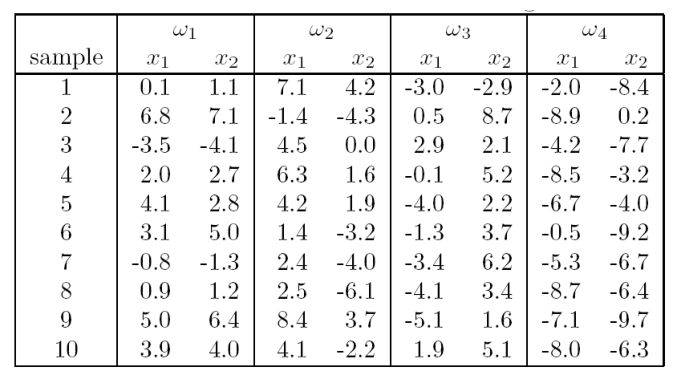
\includegraphics[width=.8\textwidth]{hw3_1.png}
%     \caption{ 数据图 }
%     \label{img1} 
% \end{figure}

$$
    \begin{array}{|c|rr|rr|rr|rr|}
        \hline           & \multicolumn{2}{|c|} {\omega_{1}} & \multicolumn{2}{c|} {\omega_{2}} & \multicolumn{2}{c|} {\omega_{3}} & \multicolumn{2}{c|} {\omega_{4}}                                 \\
        \text { sample } & x_{1}                             & x_{2}                            & x_{1}                            & x_{2}                            & x_{1} & x_{2} & x_{1} & x_{2} \\
        \hline 1         & 0.1                               & 1.1                              & 7.1                              & 4.2                              & -3.0  & -2.9  & -2.0  & -8.4  \\
        2                & 6.8                               & 7.1                              & -1.4                             & -4.3                             & 0.5   & 8.7   & -8.9  & 0.2   \\
        3                & -3.5                              & -4.1                             & 4.5                              & 0.0                              & 2.9   & 2.1   & -4.2  & -7.7  \\
        4                & 2.0                               & 2.7                              & 6.3                              & 1.6                              & -0.1  & 5.2   & -8.5  & -3.2  \\
        5                & 4.1                               & 2.8                              & 4.2                              & 1.9                              & -4.0  & 2.2   & -6.7  & -4.0  \\
        6                & 3.1                               & 5.0                              & 1.4                              & -3.2                             & -1.3  & 3.7   & -0.5  & -9.2  \\
        7                & -0.8                              & -1.3                             & 2.4                              & -4.0                             & -3.4  & 6.2   & -5.3  & -6.7  \\
        8                & 0.9                               & 1.2                              & 2.5                              & -6.1                             & -4.1  & 3.4   & -8.7  & -6.4  \\
        9                & 5.0                               & 6.4                              & 8.4                              & 3.7                              & -5.1  & 1.6   & -7.1  & -9.7  \\
        10               & 3.9                               & 4.0                              & 4.1                              & -2.2                             & 1.9   & 5.1   & -8.0  & -6.3  \\
        \hline
    \end{array}
$$

\begin{enumerate}
    \item Write a program to implement the "{\color{blue}batch perceptron}" algorithm.
          \begin{enumerate}[(a).]
              \item Starting with $\bm a = 0$, apply your program to the training data from $\omega_1$ and $\omega_2$ . Note that the
                    number of iterations required for convergence(即记录下收敛的步数)。
              \item Apply your program to the training data from $\omega_3$ and $\omega_2$ . Again, note that the number of
                    iterations required for convergence.
          \end{enumerate}
    \item Implement the {\color{blue} Ho-Kashyap algorithm} and apply it to the training data from $\omega_1$ and $\omega_3$ .
          Repeat to apply it to the training data from $\omega_2$ and $\omega_4$ . Point out the training errors, and give
          some analyses.
    \item 请写一个程序,实现 {\color{blue}MSE 多类扩展方法}。每一类用前 8 个样本来构造分类器,用后两个
          样本作测试。请给出你的正确率。
\end{enumerate}

\section*{第一部分回答}

\begin{enumerate}
    \item 由题可知:
          $$
              \begin{aligned}
                   & a = \begin{pmatrix} 0,1,0 \end{pmatrix}^T                                                                                                                       \\
                   & \omega_1:x_1 = \begin{pmatrix} 1\\4 \end{pmatrix}, x_2 = \begin{pmatrix} 2\\3 \end{pmatrix}; \omega_2:x_1 = \begin{pmatrix} 4\\1 \end{pmatrix}, x_2 = \begin{pmatrix} 3\\2 \end{pmatrix} \\
                   & 令:y_1 = \begin{pmatrix} 1\\4\\1 \end{pmatrix}, y_2 = \begin{pmatrix} 2\\3\\1 \end{pmatrix}, y_3 = -\begin{pmatrix} 4\\1\\1 \end{pmatrix}, y_4 = -\begin{pmatrix} 3\\2\\1 \end{pmatrix}          \\
              \end{aligned}
          $$
          所以:\\
          $g(y_1) = a^Ty_1 = 4 > 0$ (正确分类) , $g(y_2) = a^Ty_2 = 3 > 0$ (正确分类) ; \\
          $g(y_3) = a^Ty_3 = -1 < 0$ (错误分类) , $g(y_4) = a^Ty_4 = -2 < 0$ (错误分类) \\
          第一次修正:
          $$
              a = a + \eta_k \sum_{y\in Y(k)}y = a + y_3 + y_4 = -\left(7,2,2\right)^T
          $$
          此时:\\
          $g(y_1) = a^Ty_1 = -17 < 0 $(错误分类) , $g(y_2) = a^Ty_2 = -22 > 0$ (错误分类) ;\\
          $g(y_3) = a^Ty_3 = 32 > 0$ (正确分类) , $g(y_4) = a^Ty_4 = 27 > 0$ (正确分类) \\
          第二次修正:
          $$
              a = a + \eta_k \sum_{y\in Y(k)}y = a + y_1 + y_2 = \left(-4,5,0\right)^T
          $$
          此时:\\
          $g(y_1) = a^Ty_1 = 16 > 0 $(正确分类) , $g(y_2) = a^Ty_2 = 7 > 0$ (正确分类) ;\\
          $g(y_3) = a^Ty_3 = 11 > 0$ (正确分类) , $g(y_4) = a^Ty_4 = 2 > 0$ (正确分类) \\
          $\therefore$不再修正,$a = \left(-4,5,0\right)^T$
    \item 属于第1类的区域应该满足:$g_1(x)>g_2(x),g_1(x)>g_3(x)$ \\
          故$\omega_1$的决策面为: \\
          $g_1(x)-g_2(x) = -2x_1+1 = 0$ \\
          $g_1(x)-g_3(x) = -x_1+2x_2 = 0$ \\
          属于第2类的区域应该满足:$g_2(x)>g_1(x),g_2(x)>g_3(x)$ \\
          故$\omega_2$的决策面为: \\
          $g_2(x)-g_1(x) = 2x_1-1 = 0$ \\
          $g_2(x)-g_3(x) = x_1+2x_2-1 = 0$ \\
          属于第3类的区域应该满足:$g_3(x)>g_1(x),g_3(x)>g_2(x)$ \\
          故$\omega_3$的决策面为: \\
          $g_3(x)-g_1(x) = x_1-2x_2 = 0$ \\
          $g_3(x)-g_2(x) = -x_1-2x_2+1 = 0$ \\
          绘图如下:\\
          %   \begin{center}
          %       \begin{tikzpicture}
          %           % 修改标题样式,把标题放到图形下方
          %           \pgfplotsset{every axis title/.style={at={(0.5,-0.3)},above,yshift=6pt}}
          %           \begin{axis}[
          %                   title = {图1\quad 3分类决策面},
          %                   width = 10cm,
          %                   height = 5cm,
          %                   axis lines = middle,
          %                   ymin = -1,
          %                   ymax = 2,
          %                   xmin = -1,
          %                   xmax = 2,
          %                   xlabel = $x_{1}$,
          %                   ylabel = $x_{2}$,
          %               ]
          %               \addplot[color = red]coordinates {(0.5,-1)(0.5,1)(0.5,2)};
          %               \addplot[color = blue]{x  / 2};
          %               \addplot[color = green]{-(x - 1) / 2};
          %               \legend{$\omega_1-\omega_2$,$\omega_1-\omega_3$,$\omega_2-\omega_3$}
          %           \end{axis}
          %       \end{tikzpicture}
          %   \end{center}
          \begin{figure}[H]
              \centering
              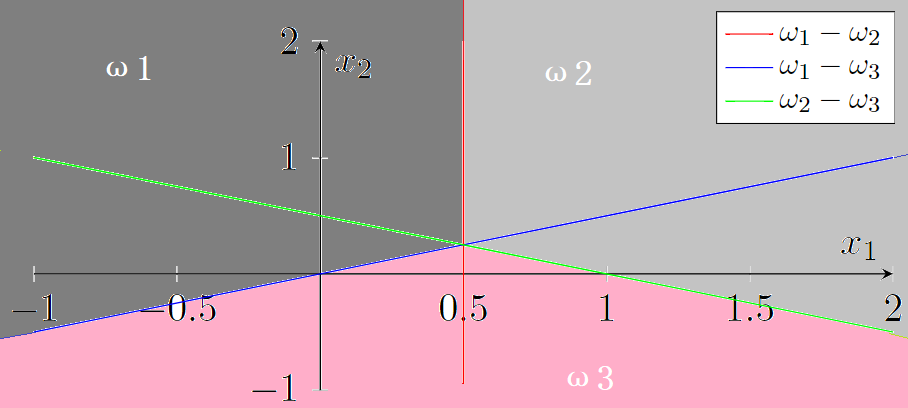
\includegraphics[width=.8\textwidth]{hw3_2.png}
              \caption{ 3分类决策面 }
              \label{img1}
          \end{figure}
          由于三条分界面交于一点(0.5,0.5),不存在不确定性区域。
\end{enumerate}

\section*{第二部分回答}

1.代码输出如下:\\
\begin{lstlisting}
Batch_perceptron algorithm:
a = [ 3.4  -3.04  3.41]
Iterations required for convergence is 24
Batch_perceptron algorithm:
a = [ 1.9  -4.14  4.86]
Iterations required for convergence is 17
Ho-Kashyap algorithm:
No solution found!
Ho-Kashyap algorithm:
a = [[0.13381828] [0.03717747] [0.01669066]]
b = [[0.46787909] [0.01      ] [0.30111691]
[0.3947414 ] [0.32167591] [0.13245664]
[0.15628159] [0.12494896] [0.50786447]
[0.24952647] [0.08073817] [0.19372309]
[0.15084515] [0.23560033] [0.18203341]
[0.03832449] [0.17504972] [0.29644592]
[0.29204113] [0.26875263]]
Iterations required for convergence is 29132
MSE准则多分类:
target = [1. 1. 2. 2. 3. 3. 4. 4.]
output = [1. 1. 2. 2. 3. 3. 4. 4.]
accuracy = 1.0
\end{lstlisting}

2.输出图像如下:\\

\begin{figure}[H]
    \begin{minipage}[t]{0.5\linewidth}
        \centering
        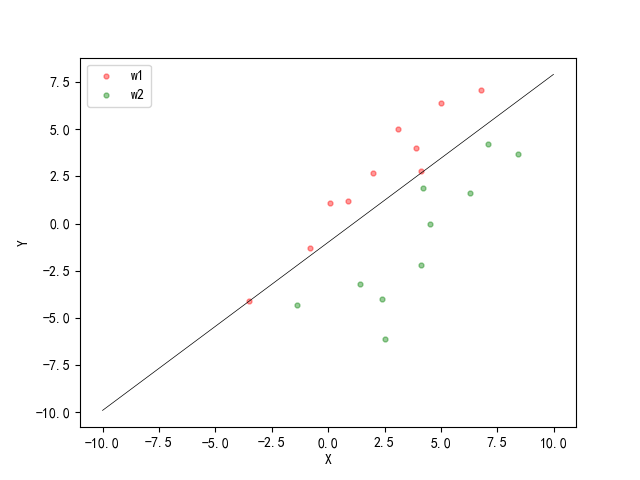
\includegraphics[width=\textwidth]{hw3_3.png}
        \caption{ $\omega_1 \quad vs\quad \omega_2$ }
    \end{minipage}%
    \begin{minipage}[t]{0.5\linewidth}
        \centering
        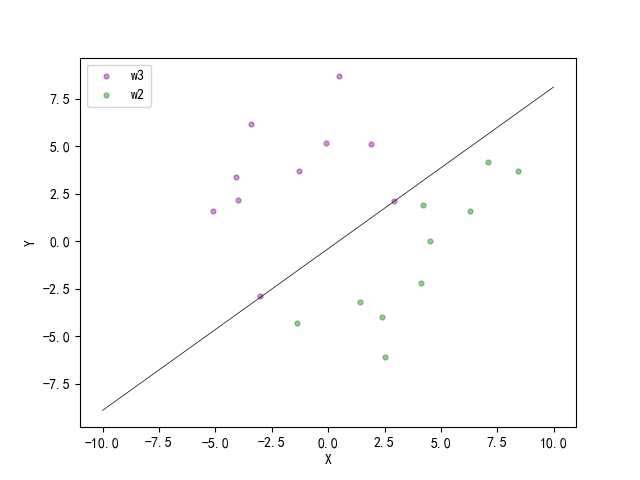
\includegraphics[width=\textwidth]{hw3_4.png}
        \caption{ $\omega_3 \quad vs\quad \omega_2$ }
    \end{minipage}
\end{figure}
\begin{figure}[H]
    \begin{minipage}[t]{0.5\linewidth}
        \centering
        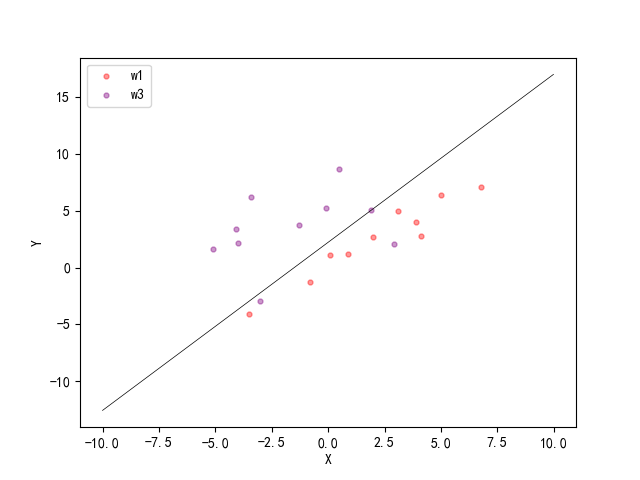
\includegraphics[width=\textwidth]{hw3_5.png}
        \caption{ $\omega_1 \quad vs\quad \omega_3$ 线性不可分 }
    \end{minipage}%
    \begin{minipage}[t]{0.5\linewidth}
        \centering
        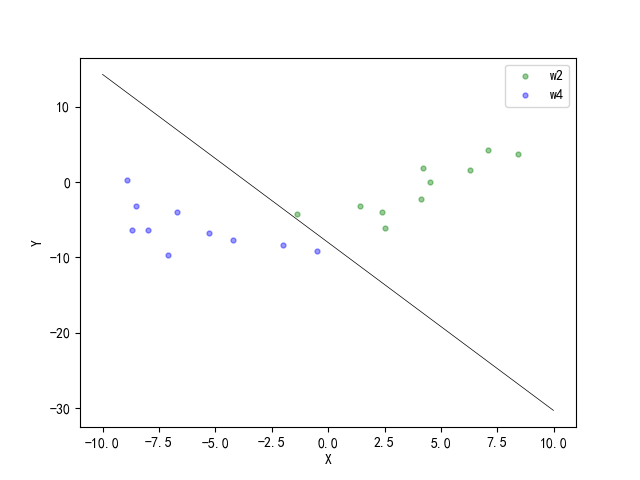
\includegraphics[width=\textwidth]{hw3_6.png}
        \caption{ $\omega_2 \quad vs\quad \omega_4$ }
    \end{minipage}
\end{figure}

3.代码见如下文件
\href{./hw3.py}{Python文件}

\end{document}